\section{Littlewood三原则}
英国数学家Littlewood在其著作\textit{Lectures on the Theory of Functions}中作出过如下总结:
\begin{itemize}
    \item 每个可测集``几乎"都是有限多个区间的和;
    \item 每个函数``几乎"都是连续的;
    \item 每个收敛的函数列都``几乎"一致收敛.
\end{itemize}
\begin{figure}[h]
    \centering
    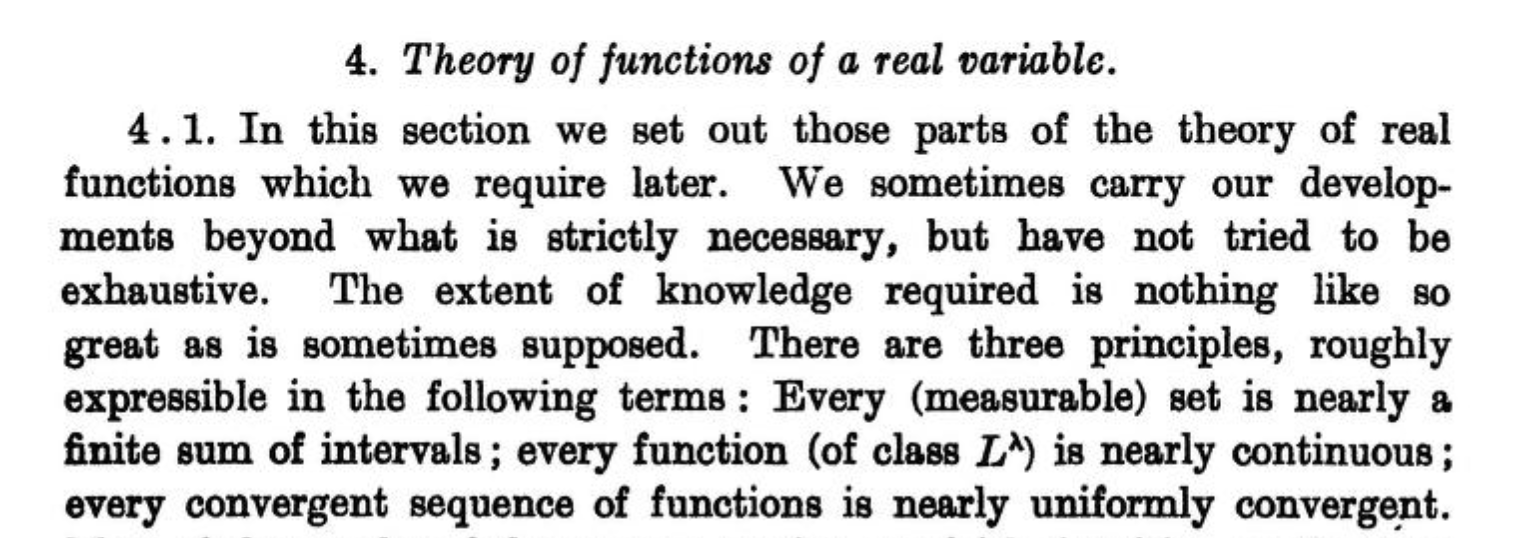
\includegraphics[scale=0.5]{image/Littlewood_3_principles.png}
    \caption{Littlewood, J. E. (1944). \textit{Lectures on the Theory of Functions}.}
    \label{fig:my_label}
\end{figure}
第一条见Lebesgue测度的正规性质, 第三条则是Egorov定理, 第二条是Lusin定理, 可借助Egorov定理推出. 我们首先复习Egorov定理的描述, 再证明Lusin定理. 
\begin{theorem}[Egorov定理]
    设$X \subset \R^d$, $m(X)<\infty$. 设定义在$X$上的可测函数列$f_n$几乎处处收敛于$f$, 则对任意$\eps>0$都存在集合$E, m(X\setminus E)< \eps$且$f_n$在$E$中一致收敛于$f$. 
\end{theorem}

Lusin定理的证明值得细细品味. 虽说这是一个关于可测函数的结论, 但证明借助了积分理论中的工具. 
